% !TeX root = ../../../main.tex
\begin{figure}[t!]
\centering
 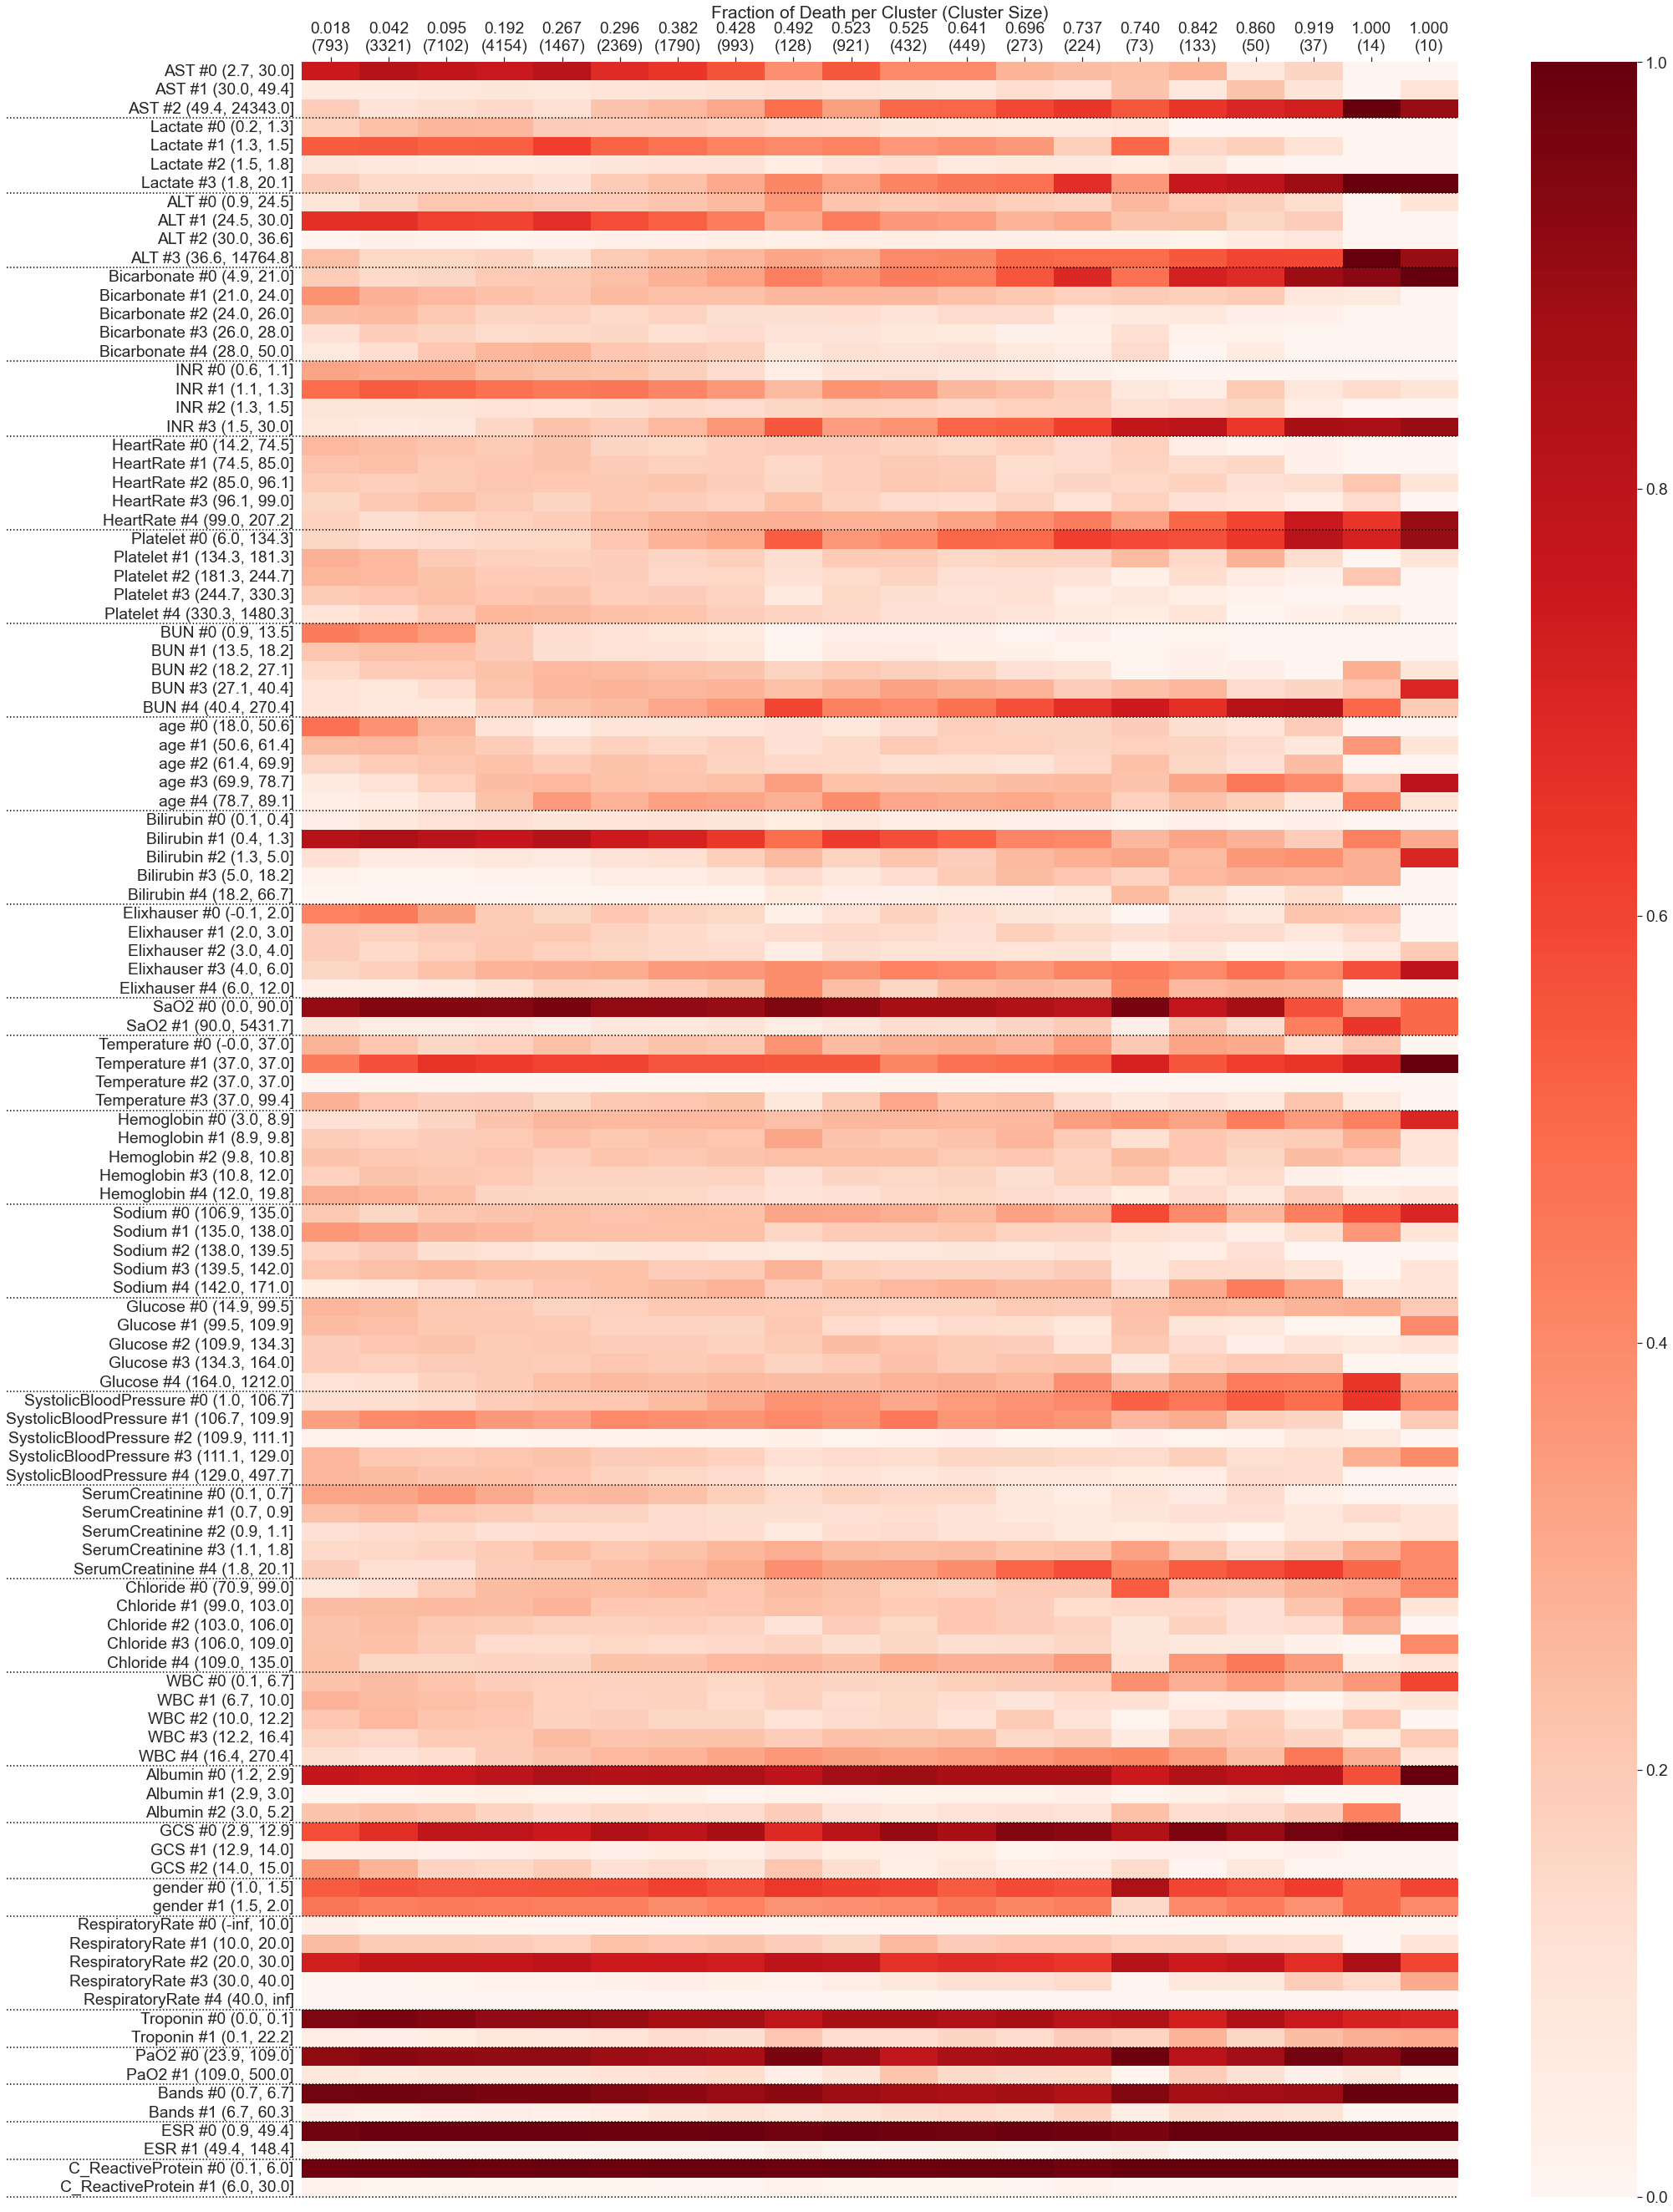
\includegraphics[width=.9\linewidth,height=0.68\textheight,keepaspectratio]{Appendices/appendix-ch02/images/mimicHeatmapFull.png}
 
  \caption{Heatmap showing how features (rows) vary across clusters (columns) for the sepsis cohort of the MIMIC dataset when using \emph{clustering on \ChTwoSmallCaps{Temporal-SCL} learned embedding space}. Heatmap intensity values can be thought of as the conditional probability of seeing a feature value (row) conditioned on being in a cluster (column); these probabilities are estimated using test set snapshots. Columns are ordered left to right in increasing fraction of test set snapshots that come from a time series that has a final outcome of death.
 }
    \ChTwoFloatLabel{ch02:fig:heatmapMIMIC_full}  
\end{figure}